% ============================================================
% LLM-BLM 実験 5：先読みのない ChronoGPT の埋め込み＋リッジ
% コンパイル：tectonic -X compile LLM-BLM_実験5.tex   （XeTeX 系。このフォルダで実行する）
% 図は 図/（作成スクリプト/figs.py が experiments/E5_chrono_embeddings/results から作る）
% 数値の出どころは experiments/E5_chrono_embeddings/results/summary.json と findings.md、
% 事前登録は experiments/E5_chrono_embeddings/preregistration.md
% ============================================================
\documentclass[xelatex,ja=standard,jafont=haranoaji,a4paper,10pt,openany]{bxjsreport}
\setpagelayout*{left=24mm,right=24mm,top=24mm,bottom=26mm,footskip=11mm}

\usepackage{amsmath,amssymb,mathtools,bm}
\usepackage{booktabs,array,multirow,longtable}
\usepackage{graphicx}
\usepackage{adjustbox}
\usepackage{xcolor}
\usepackage{tikz}
\usetikzlibrary{arrows.meta,positioning,calc,fit}
\usepackage{enumitem}
\usepackage{caption}
\usepackage{float}
\usepackage[most]{tcolorbox}
\usepackage[hidelinks,bookmarksnumbered]{hyperref}
\pdfstringdefDisableCommands{\def\Omega{Ω}\def\tau{τ}\def\Sigma{Σ}}

\graphicspath{{図/}}

\definecolor{c1}{HTML}{2A78D6}
\definecolor{c2}{HTML}{EB6834}
\definecolor{c3}{HTML}{1BAF7A}
\definecolor{c4}{HTML}{EDA100}
\definecolor{c7}{HTML}{6250D6}
\definecolor{ink2}{HTML}{52514E}
\definecolor{soft1}{HTML}{E4EEF9}
\definecolor{soft2}{HTML}{FBEEDF}
\definecolor{soft3}{HTML}{E3F3E9}
\definecolor{soft4}{HTML}{EEE8FA}
\definecolor{soft5}{HTML}{FDF3DA}

\newcommand{\code}[1]{\texttt{#1}}
\newcommand{\SP}{S\&P500}
\newcommand{\figref}[1]{図~\ref{#1}}
\newcommand{\tabref}[1]{表~\ref{#1}}
\newcommand{\chapref}[1]{第~\ref{#1}~章}
\newcommand{\secref}[1]{\ref{#1}~節}

\setlist[itemize]{leftmargin=1.6em,itemsep=0.2em,topsep=0.4em}
\setlist[enumerate]{leftmargin=1.8em,itemsep=0.2em,topsep=0.4em}
\captionsetup{font=small,labelfont=bf,skip=6pt}
\renewcommand{\arraystretch}{1.2}
\setlength{\LTpre}{6pt}
\setlength{\LTpost}{6pt}

\makeatletter
\def\@makechapterhead#1{\vspace*{0.3\Cvs}{\parindent\z@\raggedright\normalfont
  \ifnum\c@secnumdepth>\m@ne\if@mainmatter{\Large\headfont\@chapapp\thechapter\@chappos}\par\nobreak\vskip0.4\Cvs\fi\fi
  \interlinepenalty\@M\LARGE\headfont #1\par\nobreak\vskip 1.5\Cvs}}
\def\@makeschapterhead#1{\vspace*{0.3\Cvs}{\parindent\z@\raggedright\normalfont
  \interlinepenalty\@M\LARGE\headfont #1\par\nobreak\vskip 1.5\Cvs}}
\makeatother

\newtcolorbox{keybox}[1][要点]{enhanced,breakable,colback=soft1,colframe=c1,boxrule=0.5pt,arc=2pt,
  left=8pt,right=8pt,top=6pt,bottom=6pt,title={#1},fonttitle=\sffamily\bfseries\small,coltitle=white}
\newtcolorbox{notebox}[1][注意]{enhanced,breakable,colback=soft2,colframe=c2,boxrule=0.5pt,arc=2pt,
  left=8pt,right=8pt,top=6pt,bottom=6pt,title={#1},fonttitle=\sffamily\bfseries\small,coltitle=white}
\newtcolorbox{verdict}[1][判定]{enhanced,breakable,colback=soft4,colframe=c7,boxrule=0.5pt,arc=2pt,
  left=8pt,right=8pt,top=6pt,bottom=6pt,title={#1},fonttitle=\sffamily\bfseries\small,coltitle=white}

\tikzset{
  box/.style={draw=#1,fill=#1!8,rounded corners=2pt,align=center,font=\footnotesize,inner sep=4pt,
              minimum height=10mm,text width=24mm},
  arr/.style={-{Stealth[length=2mm]},color=ink2,line width=0.6pt},
}

\title{LLM-BLM 実験 5\\[6pt]
  \large 先読みのない LLM（ChronoGPT）の内部の数値に、\\過去の反応で回帰を学習させる}
\author{実験の結果の報告書}
\date{2026 年 10 月 19 日}

\begin{document}
\maketitle

% ============================================================
\chapter*{概要}
\addcontentsline{toc}{chapter}{概要}

実験 2〜4 の主役の gpt-4o-mini は、学習の期限（2023 年 10 月）より前の出来事を知っているので、2023 年 11 月以降の約 3 年にしか使えない。ChronoGPT は、年ごとに「その年の末までの文章だけ」で学習した版がある、先読みのない LLM（1.55B）である。実験 2 では、ChronoGPT に選択肢で答えさせる使い方は弱かった。今回は、作者たちの使い方にならい、ChronoGPT の内部の数値（埋め込み）を取り出し、その上に過去の反応だけで学習したリッジ回帰を置いた。手順と判定の基準は、回帰を一度も学習させる前に固定した（事前登録）。

\begin{keybox}[主な結論]
\begin{itemize}
\item \textbf{先読みのないモデルでも、2016〜2023 年の決算発表への反応を説明できた（P1 支持）。}1 標準偏差あたり $+33.6$bp（$t$ 5.5、置換の $p=0.001$）。同じ回帰の TF-IDF＋リッジは $-2.9$bp に消え、説明力は TF-IDF の約 5 倍だった。
\item \textbf{gpt-4o-mini の点数は、埋め込みのモデルに置き換えられない（P2 支持）。}同時に入れても $+111.6$bp（$t$ 8.9）で、実験 3 の 96\% が残った。
\item \textbf{ただし 1.55B の埋め込み＋線形の回帰は、gpt-4o-mini（学習なし）にも、追加学習した FinBERT にも届かない。}2023 年 11 月以降で、単独の係数は $+50$bp（FinBERT $+71$bp、gpt-4o-mini $+116$bp）。
\end{itemize}
\end{keybox}

\textbf{意味}：実験 2〜4 の「文章には反応を説明する情報がある」という結論を、先読みの疑いなしに、約 10 年で確かめられた。同じ ChronoGPT でも、選択肢で答えさせるより、内部の数値に回帰を学習させるほうがずっと強い。

\setcounter{tocdepth}{1}
{\small\tableofcontents}

% ============================================================
\chapter{目的}\label{ch:intro}

\begin{itemize}
\item \textbf{gpt-4o-mini の弱点}：2023 年 10 月までの文章で学習しているので、それより前の発表を読ませると、その後の株価の動きを知ったうえで点数を付けるおそれがある。評価できるのは 2023 年 11 月以降の約 3 年（標本 A、5,374 本）だけである。
\item \textbf{ChronoGPT}：He ほか（2025）が公開した、年ごとの版がある LLM。版 2015 は 2015 年末までの文章しか読んでいないので、2016 年以降の発表には先読みがない。
\item \textbf{実験 2 の結果}：ChronoGPT に選択肢で答えさせた点数は、標本 B（2016〜2023 年）で $+9$bp（$t$ 1.9）、標本 A でほぼ 0 と弱かった。
\end{itemize}

\begin{verdict}[問い]
\textbf{P1}：先読みのない ChronoGPT の埋め込みとリッジは、gpt-4o-mini を使えない 2016〜2023 年でも、統制を超えて反応を説明するか。\\
\textbf{P2}：2023 年 11 月以降で、gpt-4o-mini の点数は、埋め込みのモデルに置き換えられないか。
\end{verdict}

% ============================================================
\chapter{方法と事前登録}\label{ch:method}

事前登録の文書と、埋め込み・回帰・評価のコードを、コミット \code{c490cc9} に固定してから、1 回だけ実行した。実行時のコミットは \code{11b6196} で、その間の変更は「途中までの埋め込みで評価しない」ための確認（\code{5aefdec}）だけである。

\section{埋め込み}

\begin{itemize}
\item 発表文の先頭 1,792 トークン（モデルの文脈の長さ）を読ませ、最後の層の出力をトークンで平均した 1,536 個の数を、その発表の埋め込みとした。
\item 計算はこの PC の GPU で約 4.3 時間（1 本あたり約 0.4 秒）。
\end{itemize}

\section{版のそろえ方}

リッジ回帰は、学習した発表と予測する発表が同じモデルで読まれていないと意味をなさない。年ごとに違う版で読んだ数値を 1 つの回帰で混ぜると、学習と予測で物差しが変わってしまう。そこで、評価のまとまりごとに版を 1 つに固定し、学習も予測もその版で読んだ。

\begin{table}[H]
\centering
\caption{版のそろえ方。どちらも、版の期限は予測するすべての発表より前にある。}
\small
\begin{tabular}{llll}
\toprule
まとまり & 版（学習の期限） & 読んだ発表 & 予測して評価する標本 \\
\midrule
B & 2015（2015-12-31） & 2023-10 までの 15,721 本 & 標本 B：2016-01〜2023-10（14,204 本） \\
A & 2022（2022-12-31） & すべての 21,428 本 & 標本 A：2023-11〜2026-08（5,374 本） \\
\bottomrule
\end{tabular}
\end{table}

\section{リッジ回帰}

\begin{itemize}
\item 受理日の四半期ごとに、その四半期が始まる前に反応の窓が閉じた発表だけで学習し、その四半期の発表を予測した（実験 2 の TF-IDF と同じ規則）。
\item 目的変数（2 取引日の超過リターン）の丸めと標準化、1,536 個の数の標準化、罰則の強さの選択（1 つ抜きの検証）は、すべて学習の標本の中だけで行った。選ばれた罰則は $1.8\times10^4$〜$5.6\times10^4$ で、候補の端には当たっていない。
\end{itemize}

\section{評価}

\begin{itemize}
\item \textbf{P1}：実験 2 の主な回帰（数値の驚き・辞書・FinBERT・TF-IDF＋リッジ・発表前のリターン・時価総額、業種と四半期の固定効果）で、注目の変数を埋め込みの予測にした。
\item \textbf{P2}：実験 3 のモデル（実験 2 の統制＋アナリスト予想との差）に埋め込みの予測を加え、gpt-4o-mini の合成点数の係数を見た。
\item どちらも、標準誤差は発表日ごとにまとめ、同じ日の中での置換 1,000 回も行った。2 つの主な検定は Holm で補正した。
\end{itemize}

% ============================================================
\chapter{結果}\label{ch:result}

\section{P1：2016〜2023 年（標本 B）}

\begin{verdict}
\textbf{支持。}埋め込みの予測の係数は 1 標準偏差あたり $+33.6$bp（95\% 区間 $+21.6$〜$+45.5$bp、$t=5.52$、置換の片側 $p=0.001$）。
\end{verdict}

\begin{figure}[H]
\centering
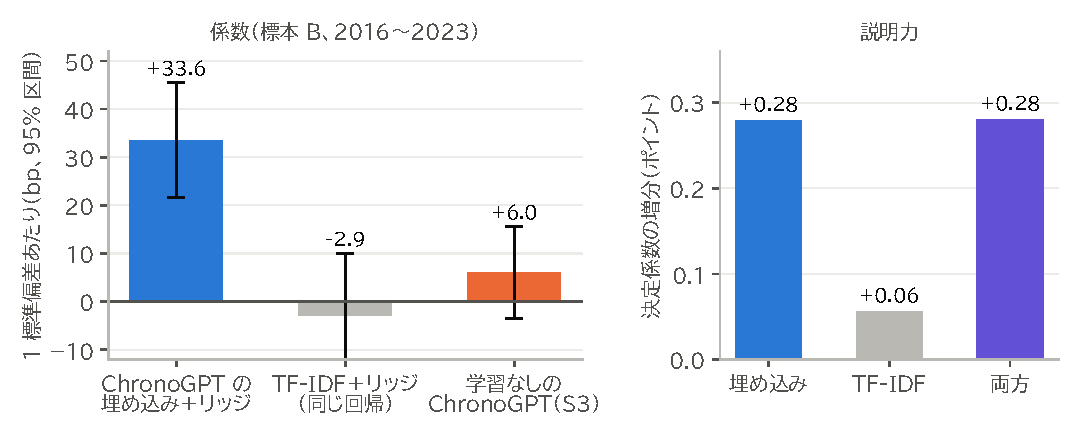
\includegraphics[width=0.95\linewidth]{block_b.pdf}
\caption{標本 B。左：係数（95\% 区間）。TF-IDF は P1 と同じ回帰の中の係数、学習なしの ChronoGPT は S3 の回帰の中の係数。右：TF-IDF を除いた統制に加えたときの決定係数の増分。}
\label{fig:b}
\end{figure}

\begin{itemize}
\item \textbf{TF-IDF を吸収した。}同じ回帰で、TF-IDF＋リッジの係数は $-2.9$bp（$t$ $-0.4$）に消えた。説明力は、埋め込みが $+0.28$ ポイント、TF-IDF が $+0.06$ ポイントで約 5 倍。両方入れても $+0.28$ で増えない（\figref{fig:b}）。反応で学習した 2 つの文章のモデルのうち、埋め込みのほうが TF-IDF の情報を含んでいる。
\item \textbf{同じモデルでも、使い方で大きく違う。}学習なしの ChronoGPT の点数は、埋め込みと同時では $+6.0$bp（$t$ 1.2）しかない。埋め込みは $+32.7$bp のまま残った（S3）。
\end{itemize}

\section{P2：2023 年 11 月以降（標本 A）}

\begin{verdict}
\textbf{支持。}埋め込みの予測と同時に入れても、gpt-4o-mini の係数は $+111.6$bp（95\% 区間 $+87.1$〜$+136.2$bp、$t=8.91$、置換の片側 $p=0.001$）。
\end{verdict}

\begin{figure}[H]
\centering
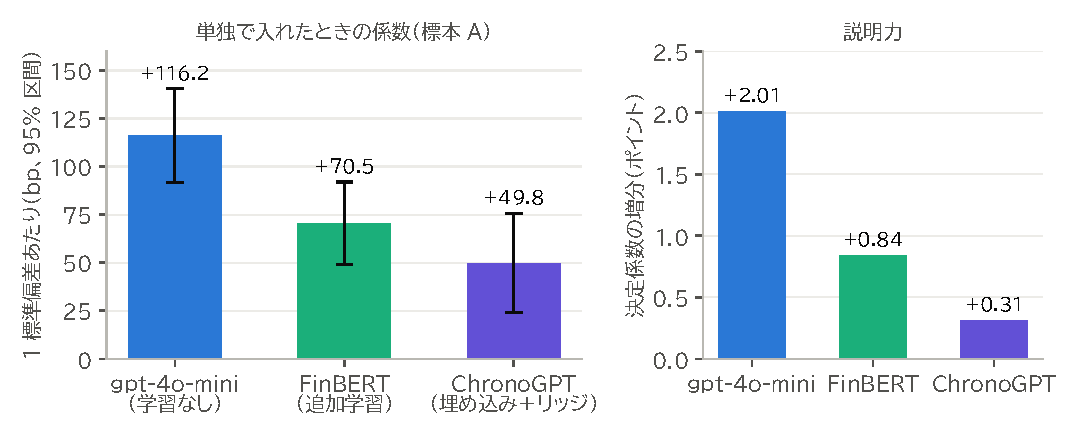
\includegraphics[width=0.95\linewidth]{sample_a.pdf}
\caption{標本 A で、それぞれを単独で実験 3 の統制に加えたときの係数（左）と決定係数の増分（右）。gpt-4o-mini は実験 3、FinBERT は実験 4、ChronoGPT は今回の S1。学習の仕方が違うので、厳密な比較ではない。}
\label{fig:a}
\end{figure}

\begin{table}[H]
\centering
\caption{副次の分析（Holm で 3 つを補正）。}
\small
\begin{tabular}{lrrr}
\toprule
& 係数 & $t$ & Holm の $p$ \\
\midrule
S1 標本 A：埋め込みだけ（gpt-4o-mini なし） & $+49.8$bp & 3.77 & $<0.001$ \\
S2 標本 A：埋め込み（gpt-4o-mini と同時） & $+21.0$bp & 1.61 & 0.054 \\
S3 標本 B：埋め込み（学習なしの ChronoGPT と同時） & $+32.7$bp & 5.40 & $<0.001$ \\
\bottomrule
\end{tabular}
\end{table}

\begin{itemize}
\item 埋め込みだけでも、標本 A で $+49.8$bp と働く。
\item ただし gpt-4o-mini と同時だと $+21.0$bp で、5\% では残らない。説明力は gpt-4o-mini が約 6.4 倍（$+2.01$ と $+0.31$ ポイント）で、順位相関は 0.43。
\item 追加学習した FinBERT（$+71$bp、$+0.84$ ポイント）にも届かない（\figref{fig:a}）。
\end{itemize}

\section{頑健性}

\begin{itemize}
\item TF-IDF を統制から除いた P1：$+32.0$bp（$t$ 5.95）。
\item すべて順位に直した版：P1 は $t$ 4.92、P2 は $t$ 6.06 で、どちらも残った。
\end{itemize}

% ============================================================
\chapter{考察と限界}\label{ch:discussion}

\section{何が分かったか}

\begin{enumerate}
\item \textbf{先読みのない LLM でも、学習させれば決算発表文から反応を読み取れる。}gpt-4o-mini を使えない 2016〜2023 年で、TF-IDF などを超えて $+34$bp。実験 2〜4 の結論が、先読みの疑いなしに約 10 年で確かめられた。
\item \textbf{使い方が大事。}同じ ChronoGPT でも、選択肢で答えさせるとほぼ効かず、内部の数値に回帰を学習させると効いた。
\item \textbf{1.55B の埋め込み＋線形の回帰には限界がある。}gpt-4o-mini（学習なし）にも、追加学習した FinBERT にも届かない。モデルの大きさか、読み方（平均した埋め込みと線形の回帰）が原因と考えられる。
\end{enumerate}

\section{次に行うこと}

\begin{itemize}
\item \textbf{ChronoGPT の中まで学習させる（LoRA）。}線形の回帰で効いたので、伸びる余地がある。版をそろえる設計はそのまま使える。
\item \textbf{月次の BLM を約 10 年で確かめる。}実験 7 の月次の BLM は 31 か月しかなく、有意でなかった。2016 年からの予測ができたので、同じ BLM を長い期間で検定できる。ただし、実験 8 のとおり、決算の情報は発表日のうちに株価に入る。
\end{itemize}

\section{限界}

\begin{itemize}
\item 版 2015 は 2015 年までの文章しか読んでいない。2020 年以降の言葉づかいに弱いかもしれないが、それでも効いた。年ごとに版を合わせる設計は、計算が約 4 倍になるので行わなかった。
\item 読むのは先頭の 1,792 トークン（約 7,000 字）。gpt-4o-mini は 15,000 字。
\item 標本 A は実験 2〜4 で、標本 B は実験 2 で一度見た期間である。
\end{itemize}

% ============================================================
\chapter*{再現の手順}
\addcontentsline{toc}{chapter}{再現の手順}

\begin{verbatim}
python experiments/E2_event_reaction/run.py       # 実験 2 の panel.csv
python experiments/E5_chrono_embeddings/embed.py  # 埋め込み（GPU 約 4.3 時間）
python experiments/E5_chrono_embeddings/run.py    # リッジと評価（1 回）
cd 資料集/02_実験/実験5_ChronoGPTの埋め込み
python 作成スクリプト/figs.py                      # この資料の図
\end{verbatim}

数値の出どころは \code{experiments/E5\_chrono\_embeddings/results/summary.json} と \code{findings.md}。埋め込みは \code{data/cache/chrono\_embeddings/}（Git の外）。費用は 0 円（この PC の GPU）。

\end{document}
